\ifx \twoside \undefined 
\documentclass[12pt,a4paper,oneside,final]{report}
\else
\documentclass[12pt,a4paper,twoside,final,openright]{report}
\fi

% Palatino
\usepackage[T1]{fontenc}
\usepackage[sc]{mathpazo}

% 한글 설정 시작
\usepackage[hangul,nonfrench,finemath]{kotex}
\usepackage[default]{dhucs-interword}
\usehangulfontspec{ut}
\usepackage[hangul]{dhucs-setspace}
\usepackage{dhucs-gremph}

\usepackage{ifpdf}
\ifpdf
  \usepackage[unicode,pdftex,colorlinks=false]{hyperref}
  \input glyphtounicode\pdfgentounicode=1
\else
  \usepackage[unicode,dvipdfm,colorlinks=false]{hyperref}
\fi
% 한글 설정 끝

% Line spacing
\usepackage{setspace}
\doublespacing
%\onehalfspacing

% Header
\pagestyle{headings}

% Bibliography
\usepackage[autostyle=true]{csquotes}
\usepackage[backend=biber,style=ieee,natbib=true,hyperref=true,backref=true,doi=false]{biblatex}
\addbibresource{wjkoh-bs-thesis.bib}
\newcommand{\Kim}{\cite{Kim:2009:SMM:1531326.1531385}} 
\newcommand{\KimKwon}{\cite{Kim:2009:SMM:1531326.1531385,Kwon:2008:GME:1360612.1360679}}
\newcommand{\Igarashi}{\cite{Igarashi:2005:ASM:1073204.1073323}} 
\newcommand{\Floater}{\cite{Floater200319}} 
\newcommand{\Hormann}{\cite{Hormann:2006:MVC:1183287.1183295}}
\newcommand{\Lipman}{\cite{Lipman:2008:GC:1360612.1360677}}

% Math
\usepackage{amsmath}
\usepackage{amssymb}
%\usepackage{array}
\providecommand{\abs}[1]{\lvert#1\rvert}
\providecommand{\norm}[1]{\lVert#1\rVert}

% Graphics
\usepackage{graphicx}

\newcommand{\thesistitle}{케이지 기반의 대규모 운동 경로 편집\\ (Cage-based Large-scale Motion Path Editing)}

\title{\thesistitle{}}
\author{고우종\\
서울대학교 컴퓨터공학부\\
\href{mailto:wjngkoh@gmail.com}{\texttt{wjngkoh@gmail.com}}
}
\date{\today}
%\keywords{Computer Graphics, Computer Animation,  Data-Driven Animation, Human Motion}

\begin{document}
%% First cover
\begin{titlepage}
\begin{center}
% Upper part of the page
{\LARGE \thesistitle{}}\\[4.0cm]

% Supervisor
{\Large 지도교수 : 이제희}\\[1.5cm]

{\Large 이 논문을 공학학사 학위 논문으로 제출함.}\\[2.5cm]

% Bottom of the page
{\Large \today}\\[1.5cm]
\vfill

% Author
\Large
서울대학교 공과대학\\
컴 퓨 터 공 학 부\\
고 우 종\\[1.0cm]
{\Large 2012년 2월}
\end{center}
\end{titlepage}

\ifx \twoside \undefined 
\else
\newpage
\phantom{placeholder} % doesn't appear on page
\thispagestyle{empty} % if want no header/footer
%\cleardoublepage
\fi

% Another cover
\maketitle

\ifx \twoside \undefined 
\else
\newpage
\phantom{placeholder} % doesn't appear on page
\thispagestyle{empty} % if want no header/footer
%\cleardoublepage
\fi

\begin{abstract}
Your abstract goes here...
\end{abstract}

\tableofcontents

\listoffigures

\chapter{서론}
\begin{figure}[htb]
\centering
%\includegraphics[width=0.8\textwidth]{image.png}
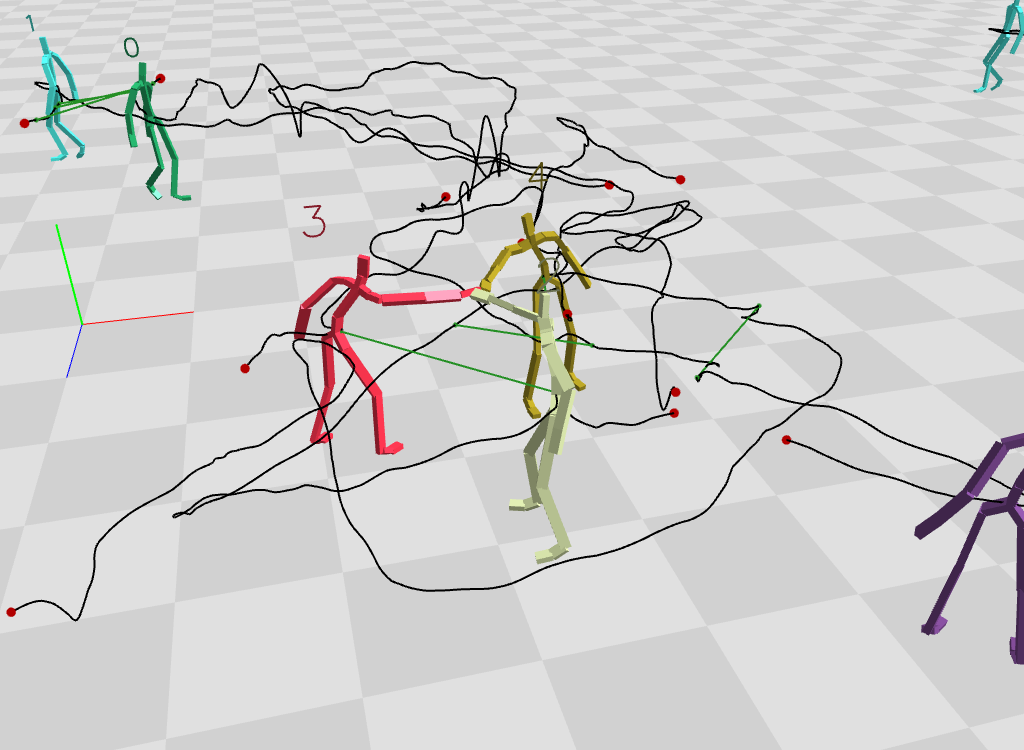
\includegraphics[width=\linewidth]{motion_path_c.png}
\caption{여러 운동 경로로 구성된 장면}
\label{fig:motion_path}
\end{figure}

최근 들어 매우 큰 규모의 군중이 등장하는 장면이 영화나 애니메이션, 비디오 게임
등에 자주 등장하고 있다. 이러한 군중 장면들은 그림~\ref{fig:motion_path}처럼
보통 등장 인물들끼리 협동 혹은 적대하는, 여러 개의 상호작용들로 구성되어 있다.
예를 들면, 여러 명의 짐꾼이 같은 물건을 동시에 들어서 옮기는 경우나 아니면 여러
명의 병사들이 서로 전투를 하고 있는 장면을 들 수 있다. 이러한 상호 작용이 운동
경로 (motion path)에 있어서는 일종의 제약조건 (constraint)으로 작용하는데, 그
이유는 바로 상호작용에 참가하는 각 캐릭터들은 해당 상호작용에 참여하는 다른
캐릭터들과 상대적인 위치, 방향, 타이밍 면에서 잘 조정되어야 하기 때문이다.  본
논문의 목표는 이러한 복잡하게 서로 의존하는 운동 경로들을 상호작용들은
유지하면서 실시간으로 편집하는 새로운 방법을 개발하는 것이다.

이 문제의 가장 근본적인 어려움은 바로 두 개의 요구사항, 즉 속도와 정확도가 서로
상충하는, 역의 관계에 있다는 것이다. 우선, 앞서 언급한 이 제약조건들을 모두
동시에 만족시키기 위해서는 운동 경로들을 편집시 매우 정확하고 총체적인 계산이
필요하다.  기존의 방식들은~\KimKwon 이 문제를 운동 경로의 모든 프레임들을 하나의 선형
시스템에 포함시킨 후 이 시스템을 풂으로써 해결하였다. 하지만 이는 질적인 품질을
높이는 대신에 이 문제의 계산 복잡도를 프레임의 총 개수에 의존하게 만듦으로써
확장 가능 (scalable)하지 않도록 만들었다. 따라서 프레임의 총 개수가 증가함에
따라 기존의 방식은 인터랙티브한 편집 속도를 달성하지 못하게 된다.

\begin{figure}[htb]
\centering
%\includegraphics[width=0.8\textwidth]{image.png}
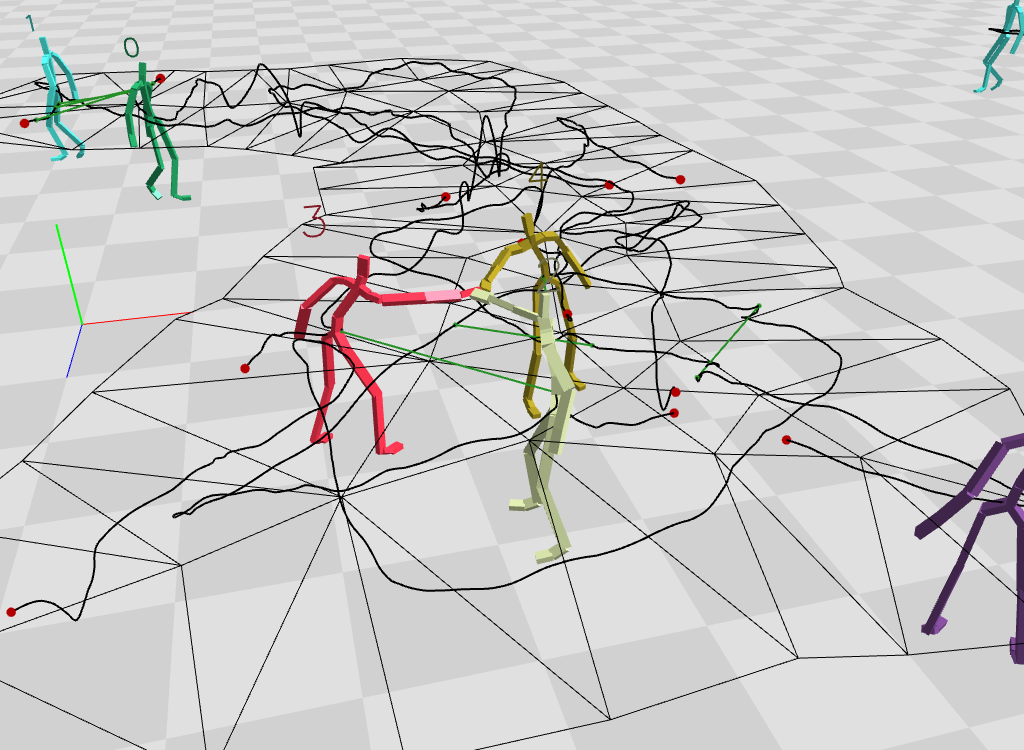
\includegraphics[width=\linewidth]{motion_path_w_mesh_c.png}
\caption{그림~\ref{fig:motion_path}에 2차원 삼각형 메시를 씌운 모습 (Delaunay)}
\label{fig:motion_path_w_mesh}
\end{figure}
 

본 논문의 가장 핵심적인 아이디어는 바로 이처럼 복잡하게 상호 종속적인 운동
경로들의 집합은 서로 분리된 꺾인 곡선들처럼 따로따로 변형되기 보다는 마치 2차원
삼각형 메시 (mesh)처럼 같이 변형된다는 것에 착안했다.  따라서 본 논문에서는
\emph{케이지 기반의 운동 경로 편집}을 이 문제의 해결책으로 제시한다. 간단히
설명하면, 먼저 여러 운동 경로들이 모인 장면에서 경로들 위에 겹치도록 오목
껍데기를 씌우고 이를 더 작은 삼각형들로 나눠서
그림~\ref{fig:motion_path_w_mesh}처럼 삼각형 메시 (mesh)를 만든다. 그리고 운동
경로의 모든 프레임의 일반화된 무게중심좌표, 예를 들면 중간값 좌표나 그린 좌표,
를 이 삼각형 메시의 외곽 꼭지점들에 대하여 계산한다. 그러고 나서 이 케이지를
가능한 한 잘 휘지 않게 (as-rigid-as-possible) 변형함으로써 그에 맞춰 변형된
운동 경로들을 계산해낼 수 있다. 다시 말해, 변형된 프레임들의 좌표는 초기 중간값
좌표 (가중치)와 변형된 후의 케이지의 외곽 꼭지점들의 좌표의 가중합 (weighted
sum)이다.

%본 논문에서 본 저자가 기여한 바는, 먼저 최대한 덜 휘게 케이지 편집법과
%중간값 좌표의 보간 (interpolation), 매끄러움 (smoothness), 그리고 선형
%정확도 (linear precision) 성질을 이용하여 기존의 계산 과정을 상당부분
%우회할 수 있다는 핵심 아이디어를 낸 것이다. 그리고 또한 실험과정 상에서 

%\section{기존}
%따라서 캐릭터들의 운동 경로 (motion path)들은 이러한 많은 제약조건, 즉 상호
%작용들에 의해 매우 복잡하게 얽혀서 서로 종속성을 강화시킨다.
%
%왜냐하면, 상호작용이 어긋나지 않도록 유지하기 위해서는 각 캐릭터들의 매
%프레임이 위치나 방향, 타이밍 면에서 다른 프레임과 맞도록 매우 미세하게
%조정되어야 하기 때문이다.  더군다나, 이러한 거대한 군중 장면의 사용은 앞으로
%자동화된 생성 방식들이 새로 개발됨에 따라 더욱 널리 사용되어질 것으로 예상된다.
%따라서 이처럼 거대한 군중 장면을 상호작용들은 최대한 그대로 유지하면서
%실시간으로 편집하는 새로운 방법이 애니메이터들에게 필요하게 되었다.

%이 문제를 해결하기 위해, 본 논문에서는 문제를 처음부터 다시 재정의하고 새로운
%접근 방식을 도입했다. 기존의 방식~\cite{Kim:2009:SMM:1531326.1531385}을
%개선시키는 것은 기존 방식의 구조상 내재된 한계에 부딪혔다.  설명하자면, 
%
%이 한계를 극복하기 위해서, 본 저자는 계산 복잡도가 프레임의 총 개수가 아닌,
%고정된 개수의 제어점에만 의존하는 새로운 방법을 고안해냈다. 또한, 더 이상
%애니메이터가 대규모의 군중 장면을 운동 경로 하나하나씩 편집할 수 없으므로,
%조작용 핸들을 새로 정의하였다.
%
%결과적으로, 본 논문에서는 새로운 대규모의 군중 장면을 편집하는 기술을 제시한다.
%이 기술은 애니메이터들에게 원래의 상호작용은 최대한 보존하면서 운동 경로를
%자유자재로 편집할 수 있도록 한다.


\chapter{관련 연구}

기존의 방식~\Kim은 라플라시안 변형 (Laplacian deformation)을 사용하여 운동
경로를 모든 제약조건들, 예를 들면 상호작용에 있어서 캐릭터의 위치, 방향, 타이밍
등을 만족시키면서 사용자가 가하는 변형에 맞도록 부드럽게 변형했다. 본
논문에서는 기존의 방법과 달리 케이지와 중간값 좌표~\Floater, 그리고 가능한 한
잘 휘지않게 2차원 삼각형 메시 변형 (2D as-rigid-as-possible mesh editing)~\Igarashi을
사용하여 구현하였다.

\section{Mean Value Coordinates} 본 논문에서는 무게중심좌표
(barycentric coordinates)의 일반화 중 하나인 중간값 좌표 (mean value
coordinates)를 사용하였다. 이 좌표는 조화함수를 위한 중간값 정리에서 착안하여
만들어진 좌표로서, 다각형의 꼭지점들에 매겨진 값들로부터 중간값들을 보간하는데
유용하다~\Floater.

무게중심좌표는 볼록다각형에는 적용할 수 있으나, 볼록하지 않은 다각형에 대해서는
일반적으로 적용할 수 없다.  반면에, 중간값 좌표는 모서리끼리 스스로 교차하지
않는, 임의의 평면다각형에 대해서도 잘 정의된다~\Hormann. 운동 경로들을 정교하게
덮기 위해서는 오목 껍데기 (concave hull)를 사용해야 하므로 중간값 좌표는 본
논문에서 다루는 문제에 사용하기에 적합하다.

중간값 좌표의 정의를 간단히 설명하면 다음과 같다. 2차원 상의 점 $x \in
\mathbb{R}^2$ 와 순환적으로 정의된 단순 다각형 (simple polygon) $[v_0, v_1,
..., v_k, v_{k+1} = v_0]$이 있다 하자. 그리고 각 $\alpha_i$를 그 다각형의 각
$\angle v_{i+1},x,v_{i}$라 하자.

\begin{align}
\lambda_i = \frac{w_i}{\sum_{j=1}^{k}w_j}, \quad w_i =
2\frac{\tan(\alpha_{i-1}/2) + \tan(\alpha_{i}/2)}{\norm{x - v_i}}
\end{align}

그러면 가중치 $(\lambda_0, ..., \lambda_k)$가 바로 $x$의 $v_0, ...  , v_k$에
대한 중간값 좌표가 된다.

\section{Green Coordinates}
그린 좌표 (Green coordinates) 역시 오목다각형에도 적용할 수 있는
무게중심좌표의 일반화 중 하나이다. 계산 과정은 조금 더 복잡하지만, 그린 좌표는
2차원에서 순수 등각사상 (pure conformal mapping)이므로 원래 운동 경로의 형태를
중간값 좌표보다 더 잘 보존하는 특성을 가지고 있다~\Lipman.

\chapter{케이지 기반의 운동 경로 변형}
\section{개괄}
먼저 대략적으로 케이지 기반의 편집을 설명하면 다음과 같이 서술할 수 있다.
먼저, 운동 경로들을 덮는 최소한의 볼록 혹은 오목 껍데기를 만들고 이를
삼각형으로 나누어서 2차원 삼각형 메시를 구성한다. 그리고 2D as-rigid-as-possible mesh
editing~\Igarashi를 사용하여 이 2차원 삼각형 메시를 사용자가 원하는 대로 변형시킨다.
이를 통해 사용자는 이 2차원 삼각형 메시의 어떤 꼭지점이라도 마음대로 움직이고 고정시킬
수 있다. 그리고 이 변형된 2차원 삼각형 메시, 정확히는 삼각형 메시의 외곽 꼭지점들로부터 그에
대응하여 변형된 운동 경로들을 계산해낼 수 있다.

조금 더 자세히 설명하면, 운동 경로들의 모든 프레임들을 이 2차원 삼각형 메시의 외곽
꼭지점들과 그 꼭지점들에 대한 일종의 무게중심좌표, 중간값 좌표나 그린 좌표, 로
표현할 수 있다. 따라서 케이지의 역할을 하는 이 2차원 삼각형 메시가 원래 형태를 최대한
유지하려고 노력하면서 변형된다면, 중간값 좌표의 보간 (interpolation), 매끄러움
(smoothness), 그리고 선형 정확도 (linear precision) 성질 덕분에 중간값 좌표로
표현된 내부의 운동 경로들 역시 부드럽게 변형된다. 새 방식은 기존의 방식과는
달리 모든 프레임이 포함된 선형 시스템을 풀 필요가 사라지므로 매우 빠른 속도로
계산을 완료할 수 있다.

\section{알고리즘}

\chapter{결과}

\begin{figure}[p]
\centering
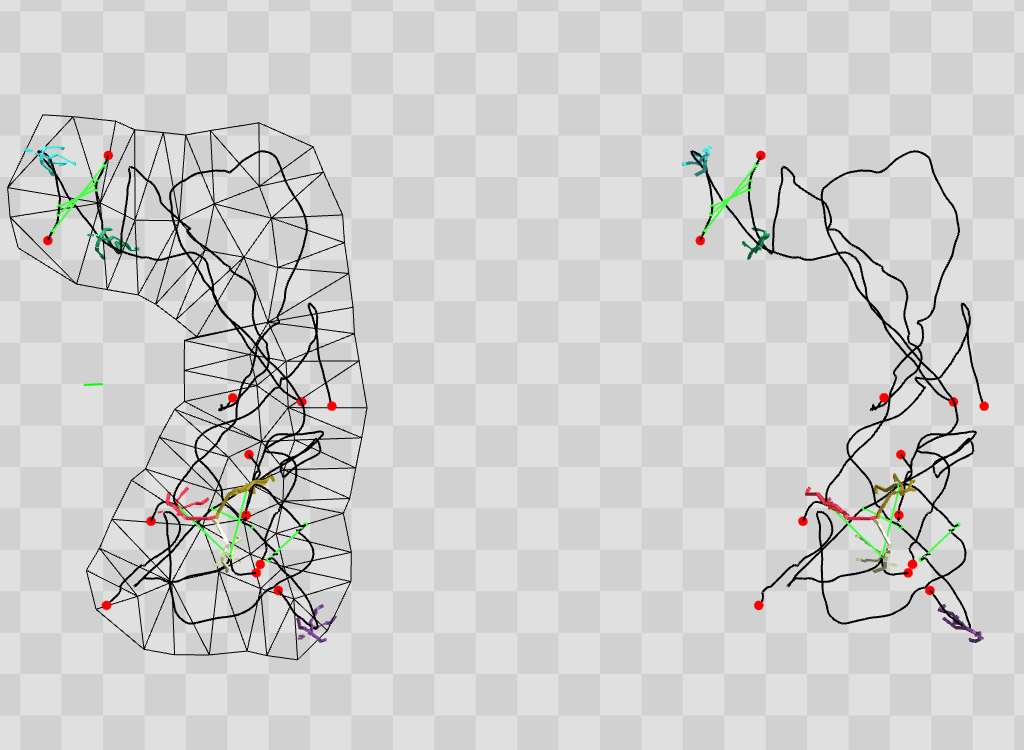
\includegraphics[width=0.9\linewidth]{before_deform_c.png}
\caption{변형 전}
\label{fig:before_deform}
\end{figure}

\begin{figure}[p]
\centering
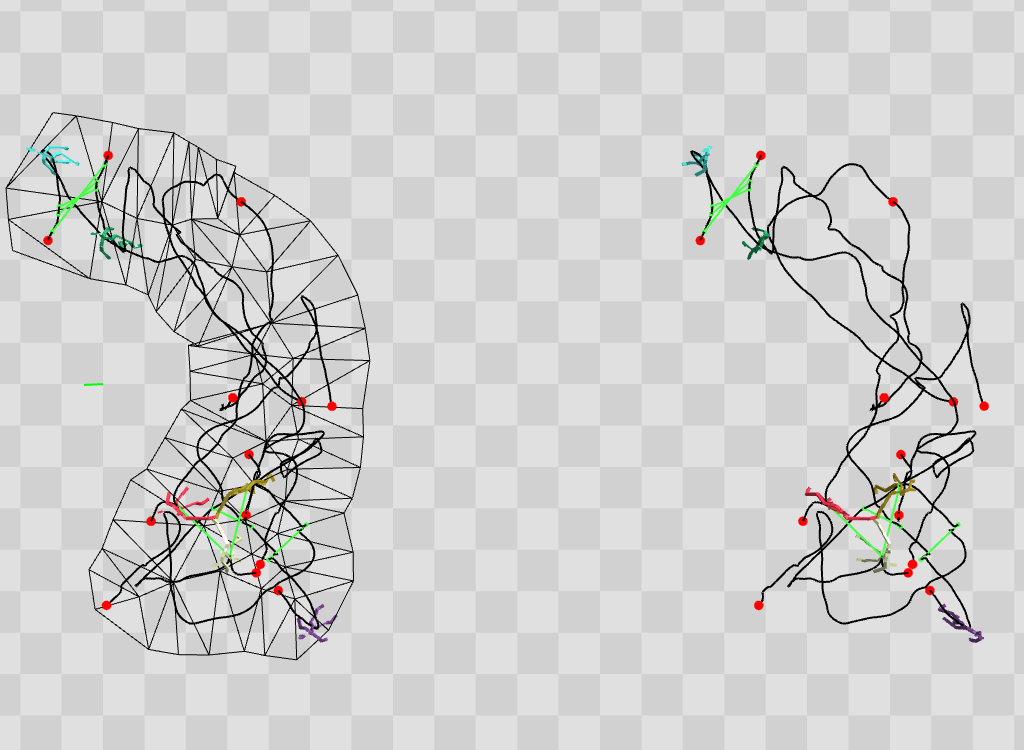
\includegraphics[width=0.9\linewidth]{after_deform_c.png}
\caption{변형 후, (좌) 본 방법 (우) 기존 Laplacian editing}
\label{fig:after_deform}
\end{figure}

\begin{table}[ht]
\centering
\begin{tabular}{r*{2}{r}c}
 & 기존 방법 & 새로운 방법 & 속도 향상 \\
\hline
1 & 1437 & 14 & 102.64 \\
2 & 1469 & 14 & 104.93 \\
3 & 1446 & 14 & 103.29 \\
4 & 1391 & 13 & 107.00 \\
5 & 1440 & 13 & 110.77 \\
6 & 1444 & 13 & 111.08 \\
7 & 1386 & 13 & 106.62 \\
8 & 1444 & 13 & 111.08 \\
9 & 1394 & 13 & 107.23 \\
10 & 1442 & 13 & 110.92 \\
\hline
평균 & 1429.3 & 13.3 & 107.55 \\
\end{tabular}
  \caption{An example of table}
  \label{my_table}
\end{table}

\chapter{결론}
결과적으로, 이 해결법을 통해 계산 복잡도를 매우 큰폭으로 낮출 수 있었고 편집
과정을 확장 가능 (scalable)하게 만들 수 있었다. 왜냐하면, 이 새로운 방식의 계산
복잡도는 모든 프레임의 개수에 의존적이지 않고 케이지의 꼭지점의 개수에
의존적이기 때문이다. 또한, 케이지라는 조작의 중간 매개체를 도입함으로써
애니메이터들이 거대한 군중 장면을 편집할 수 있도록 케이지의 꼭지점들을 새로운
조작 핸들로서 제시하였다.

%future work


\printbibliography
\end{document}
